\documentclass{beamer}
%\documentclass[xcolor=pst,dvips,epic,eepic]{beamer}

\usepackage[utf8]{inputenc}
\usetheme{Singapore}
\usepackage{xcolor}
\setbeamertemplate{footline}[frame number]

%\usepackage{pgf,pgfarrows,pgfnodes,pgfautomata,pgfheaps,pgfshade}
%\usepackage[pst]{xcolor}
%\usepackage{xxcolor}
\usepackage{mathlist}

%\usepackage[frenchb]{babel}
\usepackage[utf8]{inputenc}
\usepackage{amsmath,amssymb,amsthm}

\newtheorem{theo}{Theorem}

\usepackage{pstricks}

%\usepackage{eepic}

\usepackage{times}

%\usepackage{pst-tree}

\usepackage{ulem}

\usepackage{listings}
%\topmargin=-0.6in
\lstloadlanguages{C++}
\lstset{language=C++}
%%}

\setbeamercovered{dynamic}

\def\bxi{\boldsymbol\xi}
\def\bomega{\boldsymbol\omega}
\def\bxi{\boldsymbol\xi}

\def\rit{\mathcal{R}}

\def\cF{\mathcal{F}}
\def\cQ{\mathcal{Q}}

\author[Fabian Bastin]{Fabian Bastin \\ \url{fabian.bastin@umontreal.ca} \\ Université de Montréal -- CIRRELT -- IVADO -- Fin-ML}
\date{}
\title[Two-stage SP]{Stochastic optimization\\Two-stage stochastic programming with recourse}

% manque la caractérisation de K_2 comme polyèdre. Voir Birge & Louveaux, chapitre 2

\begin{document}

\frame{\titlepage}

\begin{frame}
	\frametitle{Formalization}
	
	Uncertainty: representation by means of {\red random elements}.
	The realizations are denoted by $\omega$, and they are drawn form the sample space $\Omega$.
	
	\mbox{}
	
	A {\red event} $A$ is a subset of $\Omega$; the collection of random of random events is denoted by $\mathcal{A}$.
	The event $A \in \mathcal{A}$ occurs if the output of the experiment is an element from $A$.
	
\end{frame}

\begin{frame}
	\frametitle{A random linear program}
	
	Consider the (toy)	problem
	\begin{align*}
	\min_x\ & x_1+x_2\\
	\mbox{s.t. } & \omega_1x_1 + x_2 \geq 7 \\
	& \omega_2x_1 + x_2 \geq 4 \\
	& x_1, x_2 \geq 0,
	\end{align*}
	where $\omega_1 \sim U[1,4]$, $\omega_2\sim U[1/3,1]$.
\end{frame}

\begin{frame}
	\frametitle{What to do?}
	
	\begin{itemize}
		\item
		How to solve this problem?
		\item
		What is the {\sl meaning} of solving this problem?
		\item
		Is it possible to decide on $x$ {\sl after} having observed the realization of the random vector $\bomega$?\\
		We then talk of an {\red wait-and-see} approach.
		The problem is then easier to solve (we have here a simple linear program).
		\item
		But this approach is rarely appropriate!!! We usually have to decide on $x$ {\red before} we know the realizations of $\bomega$!
		\item
		Usually, the ``wait-and-see'' approach is not appropriate to model the reality behavior: we have to decide on $x$ before we know the realizations from $\omega$.
		%		\item
		%It the example, we have to decide what to do before we know the realizations $\omega_1$, $\omega_2$.
		\item
		Three suggestions:
		\begin{enumerate}
			\item
			try to estimate, predict, the uncertainty;
			\item
			chance-constraints;
			\item
			penalties on deviations.
		\end{enumerate}
	\end{itemize}
	
\end{frame}

\begin{frame}
	\frametitle{A random linear program}
	
	Consider the following linear program, parametrized by the random vector $\bomega$:
	\begin{align*}
	\min_x\ & c^T x \\
	\mbox{s.t. } & Ax = b \\
	& T(\bomega)x = h(\bomega) \\
	& x \in X,
	\end{align*}
	with $X = \lbrace x \in \rit^n | l \leq x \leq u \rbrace$. Example:
	\begin{align*}
	\min_x\ & x_1+x_2\\
	\mbox{s.t. } & \omega_1x_1 + x_2 \geq 7 \\
	& \omega_2x_1 + x_2 \geq 4 \\
	& x_1, x_2 \geq 0.
	\end{align*}
\end{frame}

\begin{frame}
	\frametitle{Remove the randomness?}
	
	A popular approach consists to look for reasonable values for $\omega_1$ and $\omega_2$.
	How?
	
	\mbox{}
	
	Propositions:
	\begin{itemize}
		\item unbiased: choose the mean values for each random variable;
		\item pessimistic: choose the worst-case values for $\omega$;
		\item optimistic: choose the best-case values for $\omega$.
	\end{itemize}
	
	Each approach will deliver a different optimal solution!
	
\end{frame}

\begin{frame}
	\frametitle{Penalization of violations}
	
	Again, we have to deal with decision problems where the decision $x$ has to be taken before we know the realization of $\bomega$
	\begin{itemize}
		\item
		We nevertheless have to know the distribution of $\bomega$ over $\Omega$.
		We assume for now that $\Omega$ is finite.
		\item
		In models with recourse, the random constraints are ``soft''. They can be violated, but the violation cost will influence the choice of $x$. 
		\item
		In fact, a second stage linear program is introduced; it describes how the violated random constraints are handled.
	\end{itemize}
	
\end{frame}

\begin{frame}
	\frametitle{The new problem\ldots}
	
	In the simplest case, we can simply penalize the constraints deviations by vectors of penalty coefficients $q_+$ and $q_-$.
	\begin{align*}
	\min\ & c^Tx+q^T_+s(\bomega)+q^T_-t(\bomega) \\
	\mbox{s.t. } & Ax = b, \\
	& T(\bomega)x + s(\bomega)-t(\bomega) = h(\bomega), \\
	& x \in X.
	\end{align*}
	
	\mbox{}
	
	But it is still not possible to solve the problem!
	
\end{frame}

\begin{frame}
	\frametitle{The new optimization problem}
	
	A reasonable, and solvable, problem is then
	\begin{align*}
	\min\ & c^Tx+E_{\bomega}[q^T_+s(\bomega)+q^T_-t(\bomega)] \\
	\mbox{s.t. } & Ax = b, \\
	& T(\omega)x + s(\omega)-t(\omega) = h(\omega),\ \forall \omega
	\in \Omega \\
	& x \in X.
	\end{align*}
	\begin{itemize}
		\item
		In general, we can react in a correct (and maybe optimal) way: we have a recourse to ``correct'' the first decision once the uncertainty is removed.
		\item
		A recourse structure in linear progamming is provided by 3 elements:
		\begin{itemize}
			\item
			a set $Y \subset \rit^p$ that describes the feasible set of recourse actions, for instance $Y = \lbrace y \in \rit^p | y \geq 0 \rbrace$;
			\item
			$q$: a vector of recourse costs;
			\item
			$W$: a matrix $m \times p$, called the recourse matrix.
		\end{itemize}
	\end{itemize}
	
\end{frame}

\begin{frame}
	\frametitle{Recourse formulation}
	
	The previous considerations lead us to formulate the following program:
	\begin{align*}
	\min\ & c^Tx+E_{\bomega}[q^Ty] \\
	\mbox{s.t. } & Ax = b, \\
	& T(\omega)x + Wy(\omega) = h(\omega),\ \forall \omega
	\in \Omega \\
	& x \in X, \\
	& y \in Y,\ \forall \omega.
	\end{align*}
	
	We could have $W$ varying with the realization $\omega$.
	If $W$ is unique, as in the previous formulation, we speak of {\red fixed recourse}: the recourse does not change with the scenario.\\
	But how to decide on $y$?
	
\end{frame}

\begin{frame}
	\frametitle{Some definitions}
	
	\[
	\min_{x \in X | Ax = b} \left\lbrace c^Tx + E_{\bomega} \left[ \min_{y
		\in Y} q^T y | W y = h(\bomega) - T(\bomega)x \right] \right\rbrace.
	\]
	\begin{itemize}
		\item
		{\red Second stage function}, or {\red recourse function} (penalty) $v :
		\rit^m \rightarrow \rit$:
		\[
		v(z) \overset{def}{=} \min_{y \in Y} \lbrace q^Ty | W y = z \rbrace;
		\]
		this function describes the costs related to any vector $z$ representing the ``deviations from the random constraints $T(\omega)x = f(\omega)$''.
		\item
		{\red Expected value function}, or recourse of minimum expectation
		$\mathcal{Q} : \rit^n \rightarrow \rit$:
		\[
		\cQ(x) = E_{\bomega} [ v (h(\bomega) - T(\bomega) x)].
		\]
		It describes the expected recourse cost, for any policy $x \in \rit^n$.
	\end{itemize}
	
\end{frame}

\begin{frame}
	\frametitle{The two-stage linear stochastic problem (SP)}
	
	Using the previous definitions, we can rewrite the stochastic programming problem with recourse in terms of $x$ only:
	\[
	\min_{x \in X} \lbrace c^T x + \mathcal{Q}(x) \ |\  Ax = b \rbrace.
	\]
	It is a (nonlinear) mathematical programming problem in $\rit^n$.
	
	The properties of $\mathcal{Q}(x)$ influence the solution techniques.
	
	\mbox{}
	
	Is $\mathcal{Q}(x)$
	\begin{itemize}
		\item
		linear?
		\item
		convex?
		\item
		continuous?
		\item
		differentiable?
	\end{itemize}
	
\end{frame}

\begin{frame}
	\frametitle{Expression in terms of $y$'s}
	
	\begin{align*}
	\min_{x,\ y(\bomega)}\ & E_{\bomega} [ c^T x +
	q^T y(\bomega) ] \\
	\mbox{s.t. } & Ax = b & \mbox{first-stage constraints} \\
	& T(\omega)x + Wy(\omega) = h(\omega),\ \forall \omega \in \Omega &
	\mbox{second-stage contraints} \\
	& x \in X,\ y(\omega) \in Y.
	\end{align*}
	
	Consider the (discrete) case where $\Omega = \lbrace \omega_1,\
	\omega_2,\ldots,\omega_S \rbrace \subset \rit^r$.
	\begin{align*}
	P(\omega = \omega_s) & = p_s,\ s = 1, 2,\ldots . . . , S \\
	T_s & = T (\omega),\ h_s = h(\omega) 
	\end{align*}
	
\end{frame}

\begin{frame}
	\frametitle{Deterministic equivalent}
	
	Develop along the $S$ scenarios.
	\begin{align*}
	\min_{x, y_1, \ldots, y_S}\ & c^T x + p_1 q^T y_1 + p_2 q^T y_2 + \ldots
	p_S q^Ty_S \\
	\mbox{s.t. } & \\
	& \begin{matrix} Ax & & & & & = b\\
	T_1 x & + W y_1 & & & & = h_1 \\
	T_2 x & & + W y_2 & & & = h_2 \\
	\vdots & & & \ddots & \\
	T_S x & & & & + W y_s & = h_s
	\end{matrix} \\
	& x \in X,\ y_1 \in Y,\ y_2 \in Y,\ldots, y_s \in Y.
	\end{align*}
	
\end{frame}

\begin{frame}
	\frametitle{Deterministic equivalent (cont'd)}
	
	\begin{itemize}
		\item
		$y_s = y(\omega_s)$ is the recourse action to take if the scenario
		$\omega_s$ occurs.
		\item
		Advantage: it is a linear program.
		\item
		Drawback: it is a linear program of (very) large dimension:
		\begin{itemize}
			\item
			$n+pS$ variables;
			\item
			$m_1+mS$ constraints.
		\end{itemize}
		\item
		Advantage: the linear program matrix has a special structure (stairway shape).\\
		Can we exploit it?
	\end{itemize}
	
\end{frame}

\begin{frame}
	\frametitle{Large scale,\ldots and?}
	
	Assume that we have $r$ random variables ($\Omega \subset
	\rit^r$).
	\begin{itemize}
		\item
		Consider the following problem (source: Linderoth).
		A Telecom company want to expand its network in order to meet an unknown (random) demand.
		\item
		There are 86 unknown demands.
		Each demand is independant and take a value in a set of 7 values.
		Consequently
		\[
		S = |\Omega| = 7^{86} \approx 4.77\times10^{72}.
		\]
		\ldots number of subatomic particles in the universe!
		\item
		It can be even worse\ldots\\
		If $\Omega$ is not finite, but holds an infinite number of elements?
		It is especially true with continuous random variables.
		Our ``deterministic equivalent'' would have an infinite number of variables and constraints!
		\item
		We can solve an approximate problem, obtained by sampling over the random vector.
	\end{itemize}
\end{frame}

\begin{frame}
	\frametitle{An example (cont'd)}
	
	Consider again our toy problem
	\begin{align*}
	\min_x\ & x_1+x_2\\
	\mbox{s.t. } & \omega_1x_1 + x_2 \geq 7 \\
	& \omega_2x_1 + x_2 \geq 4 \\
	& x_1, x_2 \geq 0,
	\end{align*}
	where $\omega_1 \sim U[1,4]$, $\omega_2[1/3,1]$.
	
	\mbox{}
	
	How to build the deterministic equivalent?
	
\end{frame}

\begin{frame}
	\frametitle{Example: recourse formulation}
	
	Assume for now that $\Omega$ is finite, with $S$ scenarios.
	\begin{align*}
	\min_x\ & x_1+x_2 + \sum_{s \in S} p_s \lambda (y_{1s} + y_{2s})\\
	\mbox{s.t. } & \omega_{1s}x_1 + x_2 + y_{1s} \geq 7 \\
	& \omega_{2s}x_1 + x_2 + y_{1s} \geq 4 \\
	& x_1, x_2 \geq 0,\\
	& y_{1s}, y_{2s} \geq 0.
	\end{align*}
	
	A difficulty is therefore to decide how to construct the deterministic equivalent.
	How to choose $\lambda$?
	
	\mbox{}
	
	How to construct the scenarios?
	We can proceed with Monte Carlo sampling, with $p_s = 1/N$, $\forall s$.
	We will explore this approach in more details later.
	
\end{frame}

\begin{frame}
	\frametitle{Example: recourse formulation (cont'd)}
	
	More generally, we can build the program
	\begin{align*}
	\min_x\ & x_1+x_2 + E_{\omega}[Q(x)] \\
	\mbox{s.t. } & x_1, x_2 \geq 0,
	\end{align*}
	and
	\begin{align*}
	Q(x) &= \min_y q_1y_1 + q_2y_2 \\
	\mbox{s.t. } & \omega_1 x_1 + x_2 + y_1 \geq 7, \\
	& \omega_2 x_1 + x_2 + y_2 \geq 4.
	\end{align*}
	
\end{frame}

\begin{frame}
\frametitle{Two-stage linear programming problem, fixed recourse}

More generally, consider the problem
\[
\min c^Tx + E_{\bxi}[q(\xi)^Ty(\xi)]
\]
subject to the constraints
\begin{align*}
Ax &= b, \\
T(\xi)x + Wy(\xi) &= h(\xi) \qquad \forall \xi \in \Xi, \\
x & \in X, \\
y(\xi) & \in Y,
\end{align*}
where $\bxi$ is a random vector defined on the random space 
$(\Omega, \mathcal{F}, P)$, and $\Xi$ is the support of $\bxi$.

\mbox{}

Let
\[
Q(x, \xi(\omega)) = \min_{y \in Y} \left\lbrace q(\xi)^Ty: Wy = h(\xi) - T(\xi)x \right\rbrace.
\]
\end{frame}

\begin{frame}
\frametitle{Reformulation(s)}

\[
\min_{x \in X \,|\, Ax = b} \left\lbrace c^Tx + E_{\bxi} \left[ \min_{y \in Y} \lbrace q(\bxi)^Ty \ |\ Wy = h(\bxi) - T(\bxi)x \rbrace \right] \right\rbrace 
\]

\mbox{}

Second-stage function, or recourse function, $v: \Xi \times \rit^m \rightarrow \rit$:
\[
v(\xi, z) \overset{def}{=} \lbrace q(\xi)^Ty \ |\ Wy = z \rbrace.
\]

Given a ``policy'' $x$ and a realization of the random vector $\bxi$, $z$ measures the deviation of the first stage, i.e. $z = h(\xi) - T(\xi)x$, $v(\xi, z)$ is the minimum cost to ``correct'' the decision in order to satisfy the constraints again.

\end{frame}

\begin{frame}
\frametitle{Recourse function}

The expected recourse function, or the function of minimum expected recourse, $\mathcal{Q}: \rit^n \rightarrow \rit$, for any policy $x \in \rit^n$:
\[
\mathcal{Q} \overset{def}{=} E_{\bxi}[Q(x,\bxi)],
\]
describes the recourse cost expectation, with
\[
Q(x, \xi) = v(\xi, h(\xi)-T(\xi)x).
\]

\mbox{}

With these definitions, the problem can be rewritten as:
\[
\min_{x \in X} c^Tx + \mathcal{Q}(x) \mbox{ such that } Ax = b.
\]
It is a nonlinear program over $\rit^n$. Properties?
\end{frame}

\begin{frame}
\frametitle{Summary}

Summarize our formulations.
\[
\min_{x \in \rit^n_+ \,|\, Ax = b} \left\lbrace c^Tx + E_{\bxi} \left[ \min_{y \in \rit^p_+} \lbrace q(\xi)^Ty \ |\ Wy = h(\bxi) - T(\bxi)x \rbrace \right] \right\rbrace 
\]
\[
\min_{x \in \rit^n_+ \,|\, Ax = b} \left\lbrace c^Tx + E_{\bxi}
  \left[  v(\bxi, h(\bxi)-T(\bxi)x) \right] \right\rbrace 
\]
\[
\min_{x \in \rit^n_+ \,|\, Ax = b} \left\lbrace c^Tx + E_{\bxi} \left[ Q(x,\bxi) \right] \right\rbrace 
\]
\[
\min_{x \in \rit^n_+} \left\lbrace c^Tx + \mathcal{Q}(x)
  \ |\ Ax = b \right\rbrace 
\]

\end{frame}

\begin{frame}
\frametitle{Notations}

\begin{itemize}
\item
First-stage feasible set:
\[
K_1 = \lbrace x \in \rit^n_+ \ |\ Ax = b \rbrace.
\]
\item
Second-stage feasible set:
\[
K_2 = \lbrace x \ |\ \mathcal{Q}(x) < \infty \rbrace.
\]
\end{itemize}

\mbox{}

Therefore we can rewrite the problem as
\[
\min_x \lbrace c^Tx + \mathcal{Q}(x) \ |\ x \in K_1 \cap K_2 \rbrace.
\]

\end{frame}

\begin{frame}
\frametitle{Relatively complete recourse}

A problem is said to have a {\red relatively complete recourse} if $K_1
\subseteq K_2$.
Advantage: $\forall x$ feasible in the first stage, we have $\mathcal{Q}(x) < \infty$, so we do not have to consider the case $Q(x, \xi) = \infty$.

\mbox{}

We can also define the set of second-stage feasible points, given a realization $\xi$:
\[
K_2(\xi) = \lbrace x \ |\ Q(x,\xi) < \infty \rbrace.
\]
Define
\[
K_2^P = \cap_{\xi \in \Xi} K_2(\xi).
\]
Clearly $K_2 = K_2^P$ if $\bxi$ has a finite support.
Is it still the case when $\bxi$ follows a continuous distribution?

\end{frame}

\begin{frame}
\frametitle{Relatively complete recourse (cont'd)}

We have the following results.

\begin{theo}
If $\bxi$ has finite second order moments, $P[ \xi \ |\ Q(x,\xi) < \infty] = 1$ implies $\mathcal{Q}(x) < \infty$.
\end{theo}

In other words, we must have that $Q(x,\bxi)$ is upper bounded almost surely. Proof: technical!

\mbox{}

Reminder: almost surely, or with probability one. An event $A$ is said to occur almost surely if $P[A] = 1$.

\mbox{}

More interestingly, we have
\begin{theo}
For a stochastic program with fixed recourse, where $\bxi$ has finite second order moments, the sets $K_2$ and $K_2^p$ are the same.
\end{theo}

\end{frame}

\begin{frame}
\frametitle{Complete recourse}

The relatively complete recourse is very useful in practice and on a theoretical point of view, but it can be difficult to identify.
A particular case of relatively complete recourse can however often be identified from the structure of $W$.

\mbox{}

We say that a problem has a {\red complete recourse} if $\forall\, z \in \rit^m$, $\forall \xi$, $v(\xi, z) < +\infty$. In other terms, $\forall\, z \in \rit^m$, $\exists\, y \in \rit_+^m$ such that $Wy = z$, i.e. if the matrix $W$ satisfies
\[
\lbrace z \ |\ z=Wy,\ y \geq 0 \rbrace = \rit^m.
\]

\mbox{}

This also implies that $\forall\, x$, $T(\xi)$, $h(\xi)$, $Q(x,\xi) < \infty$, as $z = h-Tx$.

\end{frame}

\begin{frame}
\frametitle{Simple recourse}

A particular case of complete recourse is the {\red simple recourse}, for which we have
\[
W = \begin{pmatrix} I & -I \end{pmatrix},
\]
with $I$ the identiy matrix, of order $m$.

\mbox{}

In this case, the second stage program can be read as
\begin{align*}
Q(x,\xi) & = \min_y q^+(\xi)^Ty^+ + q^-(\xi)^Ty^- \\
\mbox{s.t. } & y^+ - y^- = h(\xi)-T(\xi)x,\\
& y^+,\ y^- \geq 0.
\end{align*}
That is, for $q^+(\xi) + q^-(\xi) \geq 0$, the recourse variables $y^+$ and $y^-$ can be chosen to %(non negatively)
measure the absolute violations in the stochastic constraints.

\end{frame}

\begin{frame}
\frametitle{Simple recourse (cont'd)}

\begin{theo}
Assume that the two-stage (linear) stochastic program is feasible and has a simple recourse, and that $\bxi$ has finite second-order moments.
Then $\mathcal{Q}(x)$ is finite if and only if $\boldsymbol{q}_i^+ + \boldsymbol{q}_i^- \geq 0$ with probability one.
\end{theo}

\end{frame}

\begin{frame}
\frametitle{Simple recourse (cont'd)}

\begin{proof}
{\bf $(\Rightarrow)$} 
Assume by contradiction that $\mathcal{Q}$ is finite, but for some component $i$, $q_i^+(\xi(\omega)) + q_i^-(\xi(\omega)) < 0$ for $\omega \in \Omega_1$ with $P[\Omega_1] > 0$.
Then, for any feasible $x$, for all $\omega \in \Omega_1$ with $h_i(\xi(\omega))-T_i(\xi(\omega))x > 0$, define
$$
y_i^+(\xi(\omega)) = h_i(\xi(\omega)) - T_i(\xi(\omega))x + u,\  y_i^-(\xi(\omega)) = u.
$$
Therefore, 
$$
y_i^+(\xi(\omega)) - y_i^-(\xi(\omega)) = h_i(\xi(\omega)) - T_i(\xi(\omega))x,\ y_i^+ \geq 0,\ y_i^- \geq 0.
$$
%Therefore, $y_i^+ - y_i^-$ are feasible.
Moreover, since $\mathcal{Q}$ is finite, $Q(x, \xi(\omega))$ is feasible almost surely,
so, almost surely, we can choose $y_j^+$ and $y_j^-$ feasible, $j \ne i$.

\end{proof}

\end{frame}

\begin{frame}
\frametitle{Simple recourse (cont'd)}

\begin{proof}
{\bf $(\Rightarrow)$} 

When $u \rightarrow \infty$, $Q(x, \xi(\omega)) \rightarrow -\infty$ since $q_i^+(\xi(\omega))y_i^+ + q_i^-(\xi(\omega))y_i^- \rightarrow -\infty$.

\mbox{}

A similar argument can be applied if $h_i(\xi(\omega))-T_i(\xi(\omega))x \leq 0$, by taking
$$
y_i^+(\xi(\omega)) = u,\ y_i^-(\xi(\omega)) = -h_i(\xi(\omega)) + T_i(\xi(\omega))x + u.
$$

\mbox{}

By componing these two cases, we conclude that  $\mathcal{Q}$ is not finite.
\end{proof}

\end{frame}

\begin{frame}
\frametitle{Simple recourse (cont'd)}
	
\begin{proof}

{\bf $(\Leftarrow)$}
Assume $\boldsymbol{q}_i^+ + \boldsymbol{q}_i^- \geq 0$ with probability one, $\forall i$.
Any feasible solution satisfies
$$
y^+(\xi(\omega))-y^-(\xi(\omega))=h(\xi(\omega))-T(\xi(\omega))x, \ y^+(\xi(\omega)) \geq 0,\ y^-(\xi(\omega)) \geq 0.
$$
Therefore for almost every $\omega$, $Q(x,\xi(\omega))$ is bounded below by 0, and
from the fundamental theorem of linear programming, we can choose as optimal solution
\begin{align*}
y^+(\xi(\omega)) &= \left(h(\xi(\omega))-T(\xi(\omega))x\right)^+,\\
y^-(\xi(\omega)) &= \left(-h(\xi(\omega))+T(\xi(\omega))x\right)^+,
\end{align*}
where $a^+ = \max\{0, a\}$.
\end{proof}

\end{frame}

\begin{frame}
\frametitle{Simple recourse (cont'd)}

\begin{proof}
{\bf $(\Leftarrow)$}
Thus,
\begin{align*}
Q(x,\xi(\omega)) = \sum_{i=1}^{m} & (q_i^+(\xi(\omega))(h_i(\xi(\omega))-T_i(\xi(\omega))x)^+ + \\
& q_i^-(\xi(\omega))(-h_i(\xi(\omega))+T_i(\xi(\omega))x)^+ )
\end{align*}
Consequently $Q(x,\xi(\omega))$ is finite for almost every $\omega$ and bounded below by 0.

\mbox{}

Therefore, $\mathcal{Q}(x)$ is bounded below by 0, and according to the previous results, $\mathcal{Q}(x) < \infty$. This implies that $\mathcal{Q}(x)$ is finite.
\end{proof}

\end{frame}

\begin{frame}
\frametitle{Exercise}
	
%(Birge et Louveaux, page 87)
Consider the second stage program
\[
Q(x, \xi) = \min_y \lbrace y \ |\ \xi y = 1-x, y \geq 0 \rbrace.
\]
We assume that $\bxi$ follows a triangular distribution on $[0,1]$, with $P[\bxi \leq u] = u^2$.
	
\mbox{}
	
{\blue (a)}
Is the recourse fixed? Why?
	
\mbox{}
	
The recourse is not fixed, as $W \equiv \bxi$, and therefore, $W$ is random.
Moreover, as $\xi$ can take the value 0, the transformation
\[
y = 1/\xi - x/\xi,
\]
is not properly defined on $\Xi = [0,1]$; this also means that
\[
W =
\begin{cases}
0 & \mbox{ si } \xi = 0; \\
1 & \mbox{ si } \xi \ne 0.
\end{cases}
\]
	
\end{frame}

\begin{frame}
\frametitle{Exercise (cont'd)}
	
{\blue (b)} Express $K_2(\xi)$ for all $\xi$ in $[0,1]$.
	
\mbox{}
	
We have to consider two cases: $\xi = 0$ or $\xi \in (0,1]$.
	
\mbox{}
	
{\red 1. $\xi \in (0,1]$} In this case, as $y, \xi \geq 0$, $1-x$ has to be non-negative in order to have a well-defined problem:
\[
K_2(\xi) = \lbrace x\,|\, x \leq 1 \rbrace.
\]

The value and optimal solutions are
\[
Q^*(x,\xi) = (1-x)/\xi,\quad y^*= (1-x)/\xi.
\]
	
{\red 2. $\xi=0$} There exists no $y$ such that $0.y = 1-x$, except if $x = 1$, so
\[
K_2(0) = \lbrace 1 \rbrace.
\]
	
\end{frame}

\begin{frame}
\frametitle{Exercise (cont'd)}
	
{\blue (c)} Express $K_2$, $K_2^P$ and $\mathcal{Q}$.
	
\mbox{}
	
From the previous point, we have
\[
K_2^P = \lbrace x \,|\, x \leq 1 \rbrace \cap \lbrace 1 \rbrace =
\lbrace 1 \rbrace.
\]
We also have, as $P[\xi = 0] = 0$,
\[
\mathcal{Q}(x) = \int_0^1 \frac{1-x}{\xi} 2\xi d\xi = 2(1-x), \forall
x \leq 1.
\]
Consequently $K_2^P \subset K_2 = \lbrace x \leq 1 \rbrace$.

\mbox{}

The difference comes from the fact that a point is not in $K_2^P$ as soon as it is not feasible for a given value of $\xi$, but $K_2$ does not consider unfeasible situations that occur with a null probability.
	
%	\mbox{}
	
%	\underline{Rappel}: pour un programme stochastique avec un recours%	fixe (pas le cas ici!) où $\bxi$ a des moments seconds finis, $K_2 = K_2^P$.
	
\end{frame}

\begin{frame}
\frametitle{Recourse function}

Let $y^*_1$ and $y^*_2$ be two optimal solutions of $v(\xi, z)$, associated to $z = z_1$ and $z = z_2$, respectively.
Then, the convex combination $y^*_{\alpha} = \alpha y_1^*+(1-\alpha)y_2^*$, $\alpha \in [0,1]$, is feasible with respect to $z_{\alpha} = \alpha z_1 + (1-\alpha) z_2$, as $\alpha y_1^*+(1-\alpha)y_2^* \geq 0$, and
$$
W(\alpha y_1^*+(1-\alpha)y_2^*)
= \alpha W y_1^* + (1-\alpha) W y_2^*
= \alpha z_1 + (1-\alpha) z_2 = z_{\alpha}.
$$
Moreover,
\begin{align*}
v(\xi, z_{\alpha}) & = q(\xi)^Ty_{\alpha}^* \leq
q(\xi)^T(\alpha y_1^*+(1-\alpha)y_2^*) \\
& = \alpha q(\xi)^T y_1^*+(1-\alpha)q(\xi)^Ty_2^* \\
& = \alpha v(\xi, z_1) + (1-\alpha) v(\xi, z_2).
\end{align*}
In other words, $v$ is a convex function w.r.t. $z \in \rit^m$.

%\mbox{}

%We also have the well-known property
%\begin{theo}
%If $f_1(x)$, $f_2(x)$,\ldots,$f_q(x)$ is an arbitrary collection of convex functions, then $M(x) = \max \lbrace f_1(x), f_2(x),\ldots,f_q(x) \rbrace$ is also a convex function.
%\end{theo}
\end{frame}

\begin{frame}
\frametitle{Convexity of $Q(x, \xi)$?}

\[
Q(x,\xi) = v(\xi, h(\xi)-T(\xi)x).
\]
\begin{align*}
\lambda Q(x_1, \xi) &+ (1-\lambda) Q(x_2, \xi) \\
&= \lambda v(\xi, h(\xi)-T(\xi)x_1) + (1-\lambda) v(\xi, h(\xi)-T(\xi)x_2) \\
&\geq v(\xi, \lambda (h(\xi)-T(\xi)x_1) + (1-\lambda)(h(\xi)-T(\xi)x_2)) \\
&= v(\xi, h(\xi)-T(\xi)(\lambda x_1 + (1-\lambda)x_2)) \\
&= Q(\lambda x_1 + (1-\lambda)x_2, \xi).
\end{align*}

Therefore {\red $Q(x, \xi)$ if convex} w.r.t. $x$, given $\xi$.
More generally
\begin{theo}
If $A$ if a linear transformation from $\rit^n$ to $\rit^n$, and $f(x)$ is a convex function on $\rit^m$, the composite function $(fA)(x) \overset{def}{=} f(Ax)$ is a convex function on $\rit^n$.
\end{theo}
\end{frame}

\begin{frame}
\frametitle{Convexity of second-stage function}

We have the following result (Birge and Louveaux, Chapter~3, Theorem~5).
\begin{theo}
For a stochastic program with fixed recourse, $Q(x,\xi)$ is
\begin{enumerate}[(a)]
\item
a piecewise convex linear function in $(h,T)$,
\item
a piecewise concave linear function in $q$,
\item
a piecewise convex linear function in $x$, for all $x$ in $K = K_1 \cap K_2$.
\end{enumerate}
\end{theo}

\end{frame}

\begin{frame}
\frametitle{Convexity of second-stage function (cont'd)}

\begin{proof}
In order to show convexity in (a) and (c), it is sufficient to prove that $v(\xi, z) = \min \lbrace q(\xi)^Ty \ |\ Wy = z \rbrace$ is convex, which has already been done.
We can proceed similarly to show concavity w.r.t. $q$.

The piecewise linearity follows from the fact that the number of different optimal bases for a linear program is finite.
\end{proof}

\mbox{}

{\red Convexity of the recourse?}

\[
\mathcal{Q}(x) = E_{\bxi} [Q(x,\xi)].
\]
Suppose for now that $\xi$ has a finite support, i.e. $\Xi = \lbrace \xi_1 ,
\xi_2,\ldots, \xi_m \rbrace$. Then
\[
\mathcal{Q}(x) = \sum_{i = 1}^{m} P[\bxi = \xi_i] Q(x,\xi_i).
\]
\end{frame}

\begin{frame}
\frametitle{Convexity of the recourse}

\begin{theo}
If $f(x)$ is convex, and $\alpha \geq 0$, $g(x) = \alpha f(x)$ is convex.
\end{theo}

\begin{theo}
If $f_k(x)$, $k = 1,2,\ldots,K$, are convex functions, then $g(x) = \sum_{k=1}^K f_k(x)$ is convex.
\end{theo}

$\mathcal{Q}(x)$ is therefore a convex function w.r.t. $x$.

\mbox{}

What is happening in the continuous case?

\mbox{}

We have the following result: if $g(x,y)$ is convex w.r.t. $x$, then $\int g(x,y)dy$ is convex w.r.t. $x$. Since
\[
\mathcal{Q}(x) = \int_{\Xi} Q(x,t) dF(t),
\]
{\red $\mathcal{Q}(x)$ is convex}.

\end{frame}

\begin{frame}
\frametitle{An example\ldots}

Consider the second-stage function $Q(x,\xi)$ defined as:
\begin{align*}
\min y^++y^- \mbox{ s.t. } y^+-y^- = \xi - x,\ y^+ \geq 0,\ y^- \geq 0.
\end{align*}
In other terms:
\[
y = \begin{pmatrix} y^+ \\ y^- \end{pmatrix} \quad q = \begin{pmatrix}
    1 \\ 1 \end{pmatrix}, W = \begin{pmatrix} 1 & -1 \end{pmatrix}
  \quad h(\xi) = \xi \quad T(\xi) = 1.
\]

\mbox{}

Dual:
\begin{align*}
\max\ & (\xi-x)\pi \\
\mbox{s.t. } & \pi \leq 1,\ -\pi \leq 1
\end{align*}
or
\begin{align*}
\max\ & (\xi-x)\pi \\
\mbox{s.t. } & \pi + s_1 = 1 \\
& -\pi + s_2 = 1 \\
& s_1 \geq 0,\ s_2 \geq 0
\end{align*}

\end{frame}

\begin{frame}
\frametitle{An example: optimality conditions}

The recourse is simple, and the primal-dual/KKT conditions give
\begin{align*}
\begin{pmatrix} 1 \\ 1 \end{pmatrix} & = \begin{pmatrix} 1 \\
  -1 \end{pmatrix} \pi + \begin{pmatrix} s_1 \\ s_2 \end{pmatrix} \\
y^+ - y^- & = \xi - x \\
y^+ &\geq 0,\  y^- \geq 0 \\
s_1 &\geq 0,\ s_2 \geq 0 \\
s_1y^+ & = 0,\ s_2y^- = 0.
\end{align*}

\end{frame}

\begin{frame}
\frametitle{An example (cont'd)}

\begin{itemize}
\item
The first condition implies that we cannot have
$s_1 = s_2 = 0$.
\item
From the complementarity conditions, we have that $y^+ = 0$ or $y^-
= 0$.
\item
We have to consider two cases:
\begin{itemize}
\item
$x \leq \xi$: in this situation, we have
\[
y^+ = \xi -x,\quad y^- = 0.
\]
\item
$x \geq \xi$: then,
\[
y^- = x-\xi,\quad y^+ = 0.
\]
\end{itemize}
\item
Consequently,
\[
Q(x,\xi) = \begin{cases} \xi-x & \mbox{ si } x \leq \xi, \\
x - \xi & \mbox{ si } x \geq \xi. \end{cases}
\]
\end{itemize}

\end{frame}

\begin{frame}
\frametitle{Graphically?}

Assume that $\bxi$ can take the realizations $1$, $2$, $4$.

\begin{center}
\begin{minipage}{0.9\textwidth}
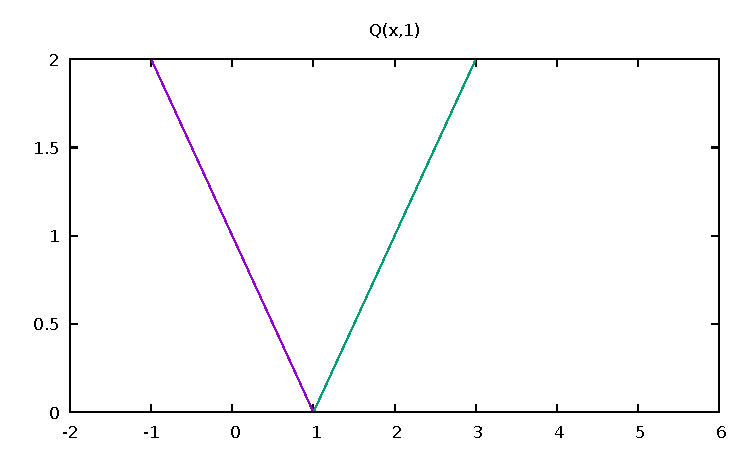
\includegraphics[width=\textwidth]{recourse_1.pdf}
\end{minipage}
\end{center}

\end{frame}

\begin{frame}
\frametitle{Graphically (cont'd)}

\begin{center}
\begin{minipage}{0.9\textwidth}
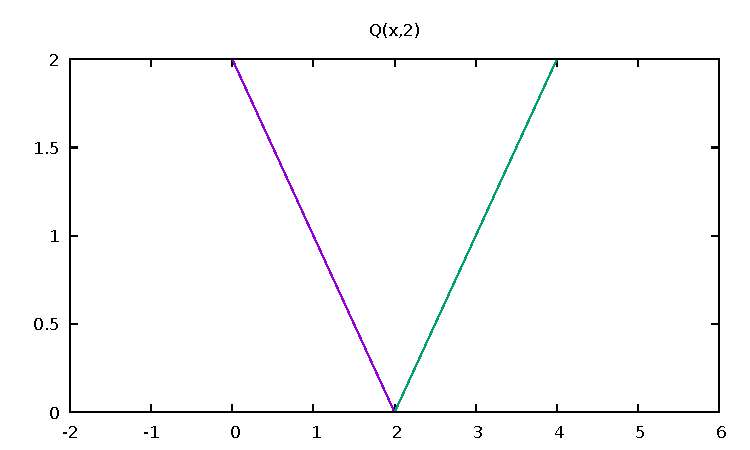
\includegraphics[width=\textwidth]{recourse_2.pdf}
\end{minipage}
\end{center}

\end{frame}

\begin{frame}
\frametitle{Graphically (cont'd)}

\begin{center}
\begin{minipage}{0.9\textwidth}
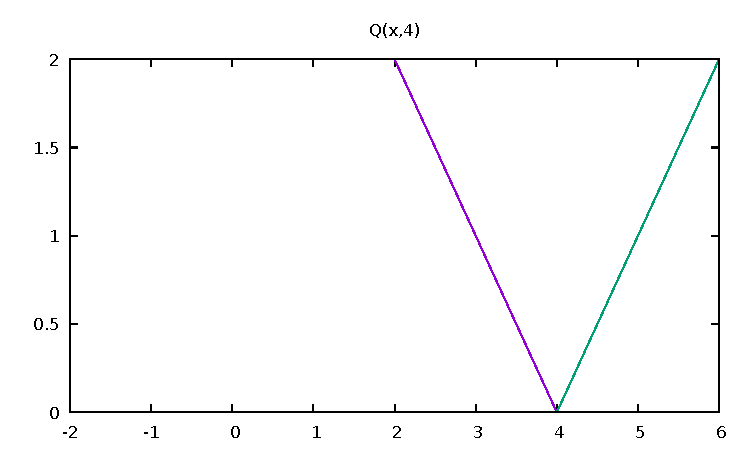
\includegraphics[width=\textwidth]{recourse_4.pdf}
\end{minipage}
\end{center}

\end{frame}

\begin{frame}
\frametitle{$\mathcal{Q}(x)$}

What about $\mathcal{Q}(x)$?

\mbox{}

Assume that the three realizations have the same probability.

\mbox{}

We have to consider 4 cases:
\begin{enumerate}
\item
$x \leq 1$: $\mathcal{Q}(x) = 7/3 - x$;
\item
$1 \leq x \leq 2$: $\mathcal{Q}(x) = 5/3-x/3$;
\item
$2 \leq x \leq 4$: $\mathcal{Q}(x) = x/3+1/3$;
\item
$4 \leq x$: $\mathcal{Q}(x) = x-7/3$;
\end{enumerate}

\end{frame}

\begin{frame}
\frametitle{Graphically}

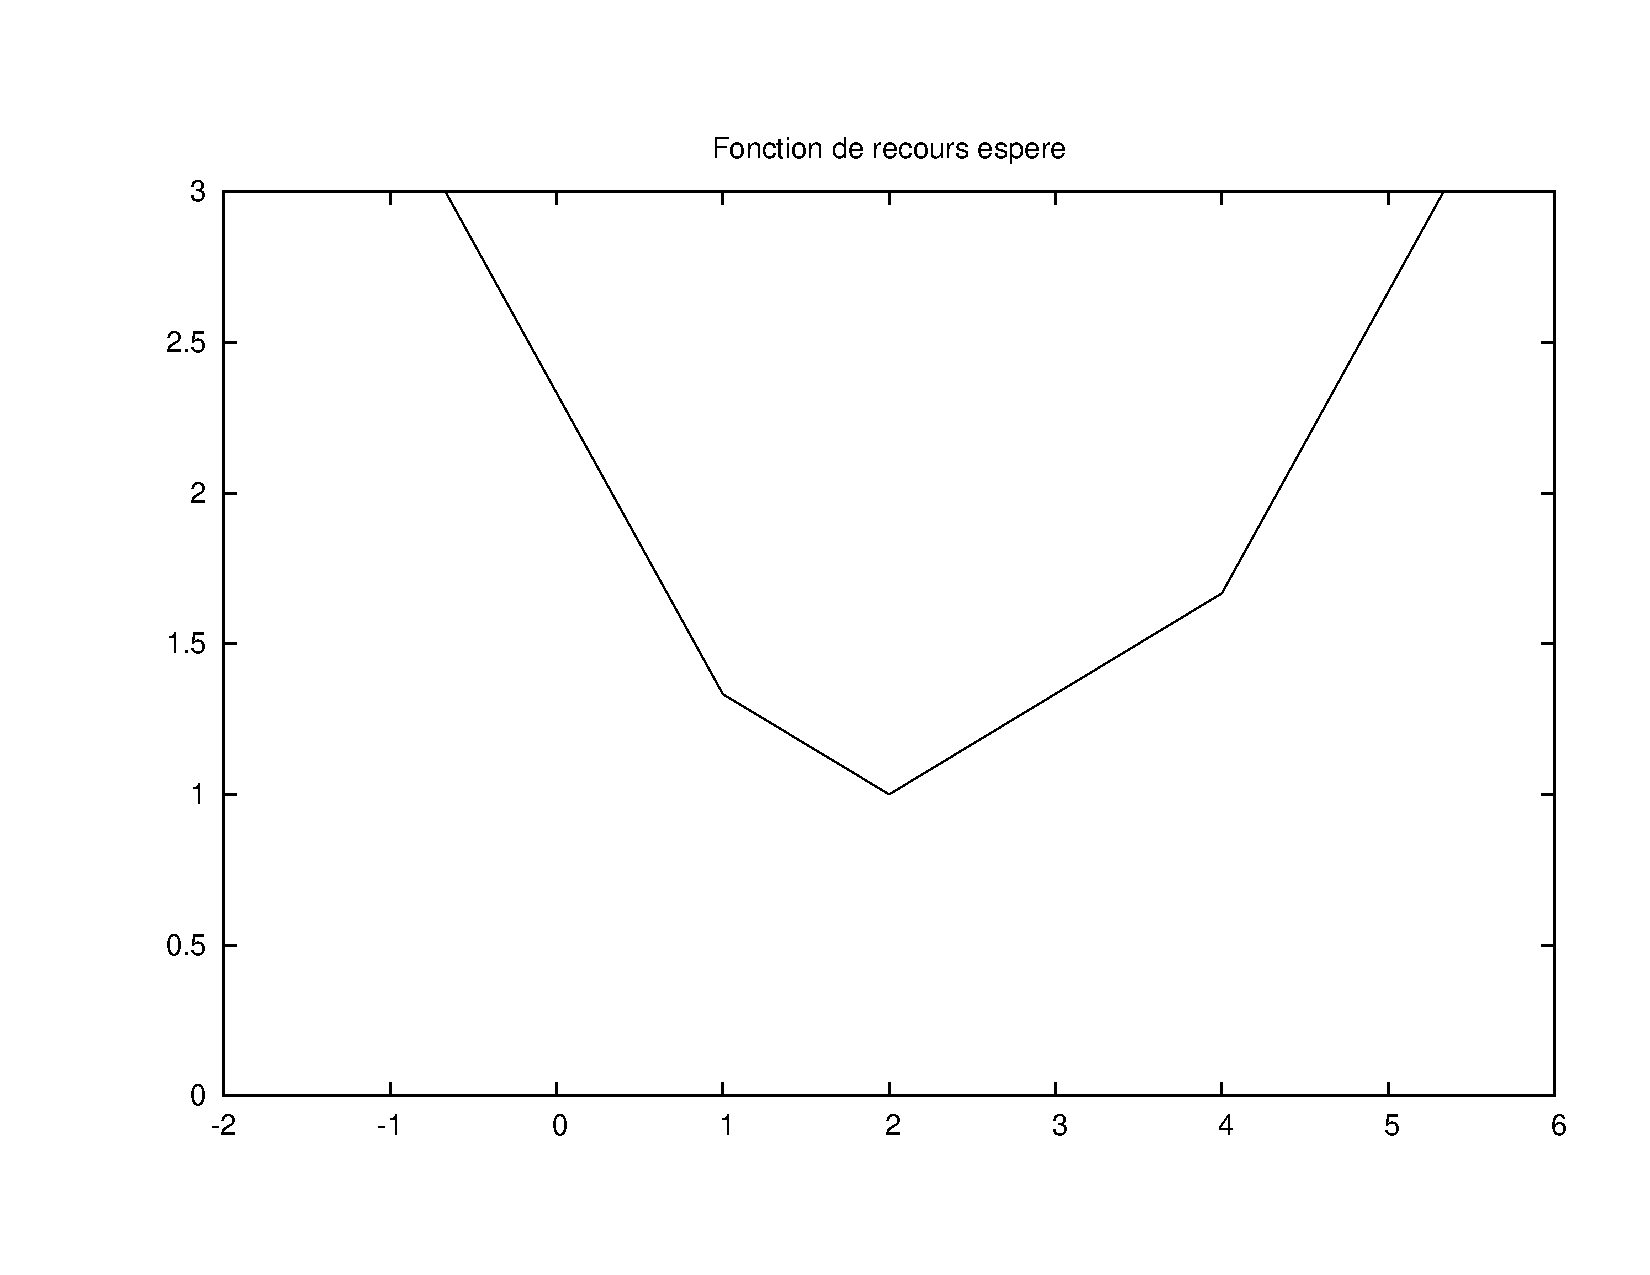
\includegraphics[width=0.9\textwidth]{recourse_all.pdf}

\end{frame}

\begin{frame}
\frametitle{Properties of $\mathcal{Q}(x)$}

We note that $\mathcal{Q}(x)$ is convex and piecewise linear.
As $\mathcal{Q}(x)$ is a finite weighted sum of piecewise linear functions when the support of $\bxi$ is finite, we have the following result.

\begin{theo}
For a stochastic program with fixed recourses where $\bxi$ has finite second-order moments,
\begin{enumerate}[(a)]
\item
$\mathcal{Q}(x)$ is a convex Lipschitz function and is finite over $K_2$;
\item
when $\bxi$ has a finite support, $\mathcal{Q}(x)$ is piecewise linear.
\end{enumerate}
\end{theo}

Reminder: a function $f$ is Lipschitz if there exists some $M < \infty$ such that for all $x$, $y$,
\[
|f(x)-f(y)| \leq M \| x-y \|.
\]

\end{frame}

\begin{frame}
\frametitle{Differentiability of the recourse}

Is $\mathcal{Q}(x)$ also differentiable?

\mbox{}

The recourse function is partially differentiable with respect to $x_j$ at $(\hat{x}, \hat{\xi})$ if the directional derivative exists for the direction $e_j$.
In other terms, there exists a function $\frac{\partial Q(x,\xi)}{\partial x_j}$ such that
\[
\frac{Q(\hat{x}+he_j,\hat{\xi}) - Q(\hat{x},\hat{\xi})}{h} =
\frac{\partial Q(x,\xi)}{\partial x_j} + \frac{\rho_j (\hat{x},
  \hat{\xi}; h)}{h},
\]
with
\[
\frac{\rho_j (\hat{x}, \hat{\xi}; h)}{h} \rightarrow 0, \mbox{ as } h\rightarrow 0.
\]

\mbox{}

We will assume from now that $\nabla_x Q(x, \xi) = \left( \frac{\partial
  Q(x,\xi)}{\partial x_1},\ldots, \frac{\partial
  Q(x,\xi)}{\partial x_n} \right)$ exists.

\end{frame}

\begin{frame}
\frametitle{Differentiability of the recourse (cont'd)}

What about the differentiability of $\mathcal{Q}(x)$?

\begin{align*}
\frac{\mathcal{Q}(\hat{x}+he_j) -
  \mathcal{Q}(\hat{x})}{h} &=
\int_{\Xi}
\frac{Q(\hat{x}+he_j,\xi) - Q(\hat{x},\xi)}{h} dP \\
&= \int_{\Xi \backslash N_{\delta}} \frac{\partial
  Q(\hat{x},\xi)}{\partial x_j} dP+ \int_{\Xi \backslash N_{\delta}}
\frac{\rho_j (\hat{x}, \xi; h)}{h} dP,
\end{align*}
where $N_{\delta}$ is measurable and $P[N_{\delta}] = 0$.
Therefore, we have
\begin{theo}
If $Q(x,\xi)$ if partially differentiable almost everywhere, if its partial derivative 
$\frac{\partial Q(\hat{x},\xi)}{\partial x_j}$ is integrable and if the residual satisfies
$(1/h) \int_{\Xi \backslash N_{\delta}} \rho_j (\hat{x}, \xi; h) dP \overset{h \rightarrow 0}{\rightarrow } 0$, then $\frac{\partial \mathcal{Q}(\hat{x})}{\partial x_j}$ exists and
\[
 \frac{\partial \mathcal{Q}(\hat{x})}{\partial x_j} =
 \int_{\Xi} \frac{\partial Q(\hat{x},\xi)}{\partial x_j} dP.
\]
\end{theo}

\end{frame}

\begin{frame}
\frametitle{Differentiability of the recourse: discrete case}

But how to prove $(1/p) \int_{\Xi
  \backslash N_{\delta}} \rho_j (\hat{x}, \xi; h) dP \overset{h
  \rightarrow 0}{\rightarrow } 0$?

\mbox{}

If we stay in the linear framework with fixed recourse, and vectors $\bxi$ with finite second-order moments, we have seen that for $\bxi$ with finite support, $\mathcal{Q}(x)$ is piecewise linear.
Therefore $\mathcal{Q}(x)$ is not differentiable.

\end{frame}

\begin{frame}
\frametitle{Differentiability of the recourse: continuous case}

If $\bxi$ is continuous, $\mathcal{Q}(x)$ is obtained as an integral over the $Q(x,\xi)$'s, that are not differentiable as they are piecewise linear given $\xi$.
However, it is $x$ that has to be fixed, not $\xi$.
It is possible to show that (the proof is quite technical)

\mbox{}

\begin{theo}
For a stochastic program with fixed recourse where $\bxi$ has finite second-order moments, if $\bxi$ is continuous, $\mathcal{Q}(x)$ is differentiable over $K_2$.
\end{theo}

\mbox{}

Intuitively, the function $\mathcal{Q}(x)$ is ``smoothed'' by the superposition of an infinite number of functions $Q(x,\xi)$.

\end{frame}

\begin{frame}
\frametitle{Two-stage non-linear problems}

Now consider the general program
\[
\min_{x \in X} E_{\bxi} [ f_0(x, \bxi) ] = \min_{x \in X}
E_{\bxi} [g_0(x,\bxi) + Q(x, \bxi)].
\]

\begin{theo}
If $g_0(\cdot,\xi)$ and $ Q(\cdot, \xi)$ are convex with respect to $x$, $\forall\ \xi \in \Xi$, and if $X$ is a convex set, the aforementioned program is convex.
\end{theo}
\begin{proof}
For $x$, $y \in X$, $\lambda \in (0,1)$ and $z = \lambda x +
(1-\lambda) y$, we have
\begin{multline*}
g_0(z, \xi) + Q(z, \xi) \\
\leq \lambda (g_0(x, \xi) + Q(x,
\xi)) + (1-\lambda)(g_0(y, \xi) + Q(y, \xi)).
\end{multline*}
The result follows by taking the expectation.
\end{proof}

\end{frame}

\begin{frame}
\frametitle{In a more standard form}

Inspired from Birge et Louveaux, Section~3.4.

\mbox{}

We consider the problem
\begin{align*}
\inf z &= f^1(x) + \mathcal{Q}(x), \\
\mbox{s.t. } & g_i^1(x) \leq 0,\ i = 1,\ldots,\overline{m}_1, \\
& g_i^1(x) = 0,\ i = \overline{m}_1+1,\ldots,m_1,
\end{align*}
where $\mathcal{Q}(x) = E_{\omega}[Q(x,\omega)]$ and
\begin{align*}
Q(x,\omega) &= \inf f^2(y(\omega), \omega), \\
\mbox{s.t. } & t_i^2(x, \omega) + g_i^2(y(\omega), \omega) \leq 0,\ i
= 1,\ldots,\overline{m}_2,\\
& t_i^2(x, \omega) + g_i^2(y(\omega), \omega) = 0,\ i =
\overline{m}_2+1,\ldots,m_2,
\end{align*}

\mbox{}

We say that the recourse is additive (why?).

\end{frame}

\begin{frame}
\frametitle{In a more standard form (cont'd)}

The functions $f^2(\cdot, \omega)$, $t_i^2(\cdot, \omega)$, and $g_i^2(\cdot, \omega)$ are continuous for any given $\omega$, and measurable w.r.t. $\omega$ for any given first argument.
This allows to prove that $Q(x,\omega)$ is measurable, and therefore that $\mathcal{Q}(x)$ is well defined.

\mbox{}

Reintroduce $K_1$, $K_2(\omega)$ and $K_2$.

\begin{align*}
K_1 & = \lbrace x \ |\ g_i^1(x) \leq 0,\ i =
1,\ldots,\overline{m}_1, \\
& \quad \qquad g_i^1(x) = 0,\ i = \overline{m}_1+1,\ldots,m_1 \rbrace, \\
K_2(\omega) & = \lbrace x \ |\ \exists\, y(\omega) \mbox{ t.q. }
 t_i^2(x, \omega) + g_i^2(y(\omega), \omega) \leq 0,\ i
= 1,\ldots,\overline{m}_2,\\
& \quad \qquad t_i^2(x, \omega) + g_i^2(y(\omega), \omega) = 0, \ i =
\overline{m}_2+1,\ldots,m_2 \rbrace, \\
K_2 & = \lbrace x \ |\ \mathcal{Q}(x) < \infty \rbrace.
\end{align*}

\end{frame}

\begin{frame}
\frametitle{Remarks}

The formulation is not yet totally general.
We will consider more general forms when we will discuss sampling techniques.

\mbox{}

Here, there is no more fixed recourse, but the first-stage decision $x$ acts separately in the constraints.
Goal: extend the previous results.

\mbox{}

Questions: convexity, differentiability, optimality.
We will also consider the concept of lower semi-continuity.

\end{frame}

\end{document}